\documentclass[letterpaper]{article} % DO NOT CHANGE THIS
\usepackage[submission]{aaai2027}  % DO NOT CHANGE THIS
% The serif, sans-serif, and monospaced fonts are loaded automatically by
% aaai2027.sty (newtxtext, helvet, courier). DO NOT add \usepackage{times},
% \usepackage{helvet}, \usepackage{courier}, or any other font package.
\usepackage[hyphens]{url}  % DO NOT CHANGE THIS
\usepackage{graphicx} % DO NOT CHANGE THIS
\urlstyle{rm} % DO NOT CHANGE THIS
\def\UrlFont{\rm}  % DO NOT CHANGE THIS
\usepackage{natbib}  % DO NOT CHANGE THIS AND DO NOT ADD ANY OPTIONS TO IT
\usepackage{caption} % DO NOT CHANGE THIS AND DO NOT ADD ANY OPTIONS TO IT
\frenchspacing  % DO NOT CHANGE THIS
%
% These are recommended to typeset algorithms but not required. See the subsubsection on algorithms. Remove them if you don't have algorithms in your paper.
\usepackage{algorithm}
\usepackage{algorithmic}

% --- TikZ Setup for Swiss Knife Architecture Diagram ---
\usepackage{tikz}
\usepackage{amsmath}
\usetikzlibrary{arrows.meta,positioning,fit,backgrounds,shapes.geometric,
                decorations.pathreplacing,calc,shadows.blur,shapes.arrows}

\definecolor{frozenblue}{RGB}{54,89,150}
\definecolor{frozenbluefill}{RGB}{223,232,246}
\definecolor{loraorange}{RGB}{196,110,32}
\definecolor{lorafill}{RGB}{250,231,213}
\definecolor{tourgreen}{RGB}{60,110,70}
\definecolor{tourfill}{RGB}{222,236,222}
\definecolor{selpurple}{RGB}{104,72,140}
\definecolor{selfill}{RGB}{233,224,242}
\definecolor{neutralgray}{RGB}{90,90,90}
\definecolor{neutralfill}{RGB}{240,240,240}

\tikzset{
  frozenbox/.style={rectangle, rounded corners=2pt, draw=frozenblue, thick,
    fill=frozenbluefill, minimum width=2.6cm, minimum height=1.05cm,
    align=center, font=\scriptsize},
  lorabox/.style={rectangle, rounded corners=2pt, draw=loraorange, thick,
    fill=lorafill, minimum width=2.6cm, minimum height=1.05cm,
    align=center, font=\scriptsize},
  tourbox/.style={rectangle, rounded corners=2pt, draw=tourgreen, thick,
    fill=tourfill, minimum width=2.9cm, minimum height=1.15cm,
    align=center, font=\scriptsize},
  selbox/.style={rectangle, rounded corners=2pt, draw=selpurple, thick,
    fill=selfill, minimum width=2.9cm, minimum height=1.15cm,
    align=center, font=\scriptsize},
  databox/.style={rectangle, rounded corners=1pt, draw=neutralgray,
    fill=neutralfill, minimum width=2.2cm, minimum height=0.85cm,
    align=center, font=\scriptsize},
  decision/.style={diamond, draw=selpurple, thick, fill=selfill, aspect=2.4,
    align=center, font=\scriptsize, inner sep=1pt},
  flow/.style={-{Stealth[length=2mm]}, thick, draw=neutralgray},
  loopflow/.style={-{Stealth[length=2mm]}, thick, draw=neutralgray, dashed},
  groupbg/.style={rounded corners=6pt, draw=none, fill=black!4},
  lockicon/.style={font=\scriptsize\bfseries, frozenblue}
}

%
% These are recommended to typeset listings but not required. See the subsubsection on listing. Remove this block if you don't have listings in your paper.
\usepackage{newfloat}
\usepackage{listings}
\DeclareCaptionStyle{ruled}{labelfont=normalfont,labelsep=colon,strut=off} % DO NOT CHANGE THIS
\lstset{%
	basicstyle={\footnotesize\ttfamily},% footnotesize acceptable for monospace
	numbers=left,numberstyle=\footnotesize,xleftmargin=2em,% show line numbers, remove this entire line if you don't want the numbers.
	aboveskip=0pt,belowskip=0pt,%
	showstringspaces=false,tabsize=2,breaklines=true}
\floatstyle{ruled}
\newfloat{listing}{tb}{lst}{}
\floatname{listing}{Listing}

%
% Recommended for better-looking tables
\usepackage{booktabs}

%
% Keep the \pdfinfo as shown here. There's no need
% for you to add the /Title and /Author tags.
\pdfinfo{
/TemplateVersion (2027.1)
}

% DISALLOWED PACKAGES
% \usepackage{authblk} -- This package is specifically forbidden
% \usepackage{balance} -- This package is specifically forbidden
% \usepackage{CJK} -- This package is specifically forbidden
% \usepackage{float} -- This package is specifically forbidden
% \usepackage{flushend} -- This package is specifically forbidden
% \usepackage{fullpage} -- This package is specifically forbidden
% \usepackage{geometry} -- This package is specifically forbidden
% \usepackage{hyperref} -- This package is specifically forbidden
% \usepackage{navigator} -- This package is specifically forbidden
% (or any other package that embeds links such as navigator or hyperref)
% \usepackage{indentfirst} -- This package is specifically forbidden
% \usepackage{layout} -- This package is specifically forbidden
% \usepackage{multicol} -- This package is specifically forbidden
% \usepackage{nameref} -- This package is specifically forbidden
% \usepackage{savetrees} -- This package is specifically forbidden
% \usepackage{setspace} -- This package is specifically forbidden
% \usepackage{stfloats} -- This package is specifically forbidden
% \usepackage{tabu} -- This package is specifically forbidden
% \usepackage{titlesec} -- This package is specifically forbidden
% \usepackage{tocbibind} -- This package is specifically forbidden
% \usepackage{ulem} -- This package is specifically forbidden
% \usepackage{wrapfig} -- This package is specifically forbidden
% DISALLOWED COMMANDS
% \nocopyright -- Your paper will not be published if you use this command
% \addtolength -- This command may not be used
% \balance -- This command may not be used
% \baselinestretch -- Your paper will not be published if you use this command
% \clearpage -- No page breaks of any kind may be used for the final version of your paper
% \columnsep -- This command may not be used
% \newpage -- No page breaks of any kind may be used for the final version of your paper
% \pagebreak -- No page breaks of any kind may be used for the final version of your paper
% \pagestyle -- This command may not be used
% \tiny -- This is not an acceptable font size.
% \vspace{- -- No negative value may be used in proximity of a caption, figure, table, section, subsection, subsubsection, or reference
% \vskip{- -- No negative value may be used to alter spacing above or below a caption, figure, table, section, subsection, subsubsection, or reference

\setcounter{secnumdepth}{0} %May be changed to 1 or 2 if section numbers are desired.

% The file aaai2027.sty is the style file for AAAI Press
% proceedings, working notes, and technical reports.
%

% Title

% Your title must be in mixed case, not sentence case.
% That means all verbs (including short verbs like be, is, using,and go),
% nouns, adverbs, adjectives should be capitalized, including both words in hyphenated terms, while
% articles, conjunctions, and prepositions are lower case unless they
% directly follow a colon or long dash
\title{Swiss Knife: Plug-and-Play Alignment Blades via Tournament Sampling in Speculative Decoding}
\author{
    Anonymous Submission
}
\affiliations{
    Anonymous Institution
}

%Example, Single Author, ->> remove \iffalse,\fi and place them surrounding AAAI title to use it
\iffalse
\title{My Publication Title --- Single Author}
\author {
    Author Name
}
\affiliations{
    Affiliation\\
    Affiliation Line 2\\
    name@example.com
}
\fi

\iffalse
%Example, Multiple Authors, ->> remove \iffalse,\fi and place them surrounding AAAI title to use it
\title{My Publication Title --- Multiple Authors}
\author {
    % Authors
    First Author Name\textsuperscript{\rm 1,\rm 2}\equalcontrib,
    Second Author Name\textsuperscript{\rm 2}\equalcontrib,
    Third Author Name\textsuperscript{\rm 1}\corresponding
}
\affiliations {
    % Affiliations
    \textsuperscript{\rm 1}Affiliation 1\\
    \textsuperscript{\rm 2}Affiliation 2\\
    firstAuthor@affiliation1.com, secondAuthor@affilation2.com, thirdAuthor@affiliation1.com
}
\fi


\begin{document}

\maketitle

\begin{abstract}
Alignment today is still checkpoint-bound: most pipelines implicitly hard-code a single behavioral compromise into a trained model, making it costly to revise, specialize, or hot-fix behavior after deployment (e.g., higher helpfulness, stronger harmlessness, or a different refusal posture). While instruction-conditioned switching can increase controllability, it still assumes a single frozen policy must internalize multiple behavioral regimes and remain stable under interference and distribution shift. We take a step beyond frozen-backbone switching by externalizing alignment into a changeable decode-time head. We introduce Swiss Knife, a protocol that repurposes the architecture of speculative decoding into an alignment socket: a fast draft model generates candidates, while a separately trainable auditor model enforces a chosen alignment objective during generation.

Swiss Knife's key algorithmic component is Swiss-system tournament sampling. At each decoding step, the draft model proposes a candidate set which competes in an efficient Elo-rating tournament. Rather than relying on an auditor for a hard acceptance decision, the winning candidate is chosen via a softmax draw that combines its tournament rating with an uncertainty-penalized blade score, and is accepted unconditionally. This yields stable preference-based selection while mitigating degenerate solutions such as refuse-always or templated ``safe'' boilerplate. Crucially, Swiss Knife supports objective-specific auditor ``blades''---such as helpfulness and harmlessness---that can be tuned, swapped, and updated independently of the backbone, enabling rapid post-deployment alignment updates without retraining the generator. We formalize Swiss Knife as decode-time policy shaping that combines Elo tournament ratings with uncertainty-weighted blade scores. Swiss Knife delivers stronger multi-regime alignment under comparable compute budgets,demonstrating that modular auditor heads provide a practical, updatable, and deployment-friendly path to switchable alignment.
\end{abstract}

\begin{links}
    \link{Code}{https://anonymous.placeholder/code}
\end{links}

\section{Introduction}

The predominant paradigm for aligning large language models with human values, such as Direct Preference Optimisation~\cite{rafailov2023direct} and its variants, encodes behavioural objectives directly into model weights during training. While effective, this approach remains rigid: revising a safety posture or adapting to a new deployment context demands a costly fine-tuning run and a subsequent deployment cycle.

A growing body of work addresses this inflexibility by enforcing alignment at decode time. Notable examples include ARGS by Khanov et al.~\cite{khanov2024args} and MOD by Shi et al.~\cite{shi2024mod}. These methods leave the generator model frozen and steer its output during inference via an external signal. However, existing approaches share a structural vulnerability: alignment quality is measured on an \emph{absolute} scale. Whether adding a reward gradient to logits as in ARGS or blending distributions as in MOD, systematic miscalibration of the reward model propagates directly into candidate selection. A reward model that systematically over-scores refusal tokens will drive an argmax-based decoder toward perpetual refusal. We term these \emph{reward-maximisation degeneracies}.

We propose that the root cause of these degeneracies lies in the reliance on deterministic point-estimates. When a reward model encounters out-of-distribution refusal tokens, it often produces overconfident, inflated scores that point-estimate aggregators blindly exploit. Swiss Knife, by contrast, relies on probabilistic pairwise comparisons. By modeling candidate rewards as distributions and resolving matches via a Thurstonian Case-V framework, high-reward but highly uncertain candidates have their win margins compressed toward 50\%. This structural stochasticity acts as a natural regularizer against reward-maximisation degeneracies, preventing overconfident but flawed candidates from dominating the selection process.

We formalise this insight as \textbf{Swiss Knife}. Swiss Knife structures candidate selection as a Swiss-system tournament. A small drafter model samples candidate continuations which subsequently compete in an Elo-rating tournament. Matches are decided probabilistically based on reward differences and uncertainty, preventing premature convergence to overconfident but flawed candidates. The winning candidate is then selected unconditionally via a softmax draw that factors in both the final Elo rating and an uncertainty-penalised blade score. Alignment objectives are encapsulated in \textbf{blades}: lightweight LoRA adapters~\cite{hu2021lora} trained via Direct Preference Optimisation. These blades can be hot-swapped in constant time, perfectly matching the operational reality of deployed systems that require distinct behavioural modes without retraining the generator.

\paragraph{Contributions.}
We make the following contributions:
\begin{enumerate}
    \item \textbf{Tournament-based decode-time alignment.} We introduce the Tournament Sampling Auditor (TSA) as a probabilistic candidate selection rule that dampens reward overconfidence, demonstrating empirical resistance to refusal collapse on the HH-RLHF benchmark (the Experiments section).
    \item \textbf{Uncertainty-weighted objective.} We propose a selection criterion that penalizes candidates with high reward uncertainty, providing an efficient log-ratio proxy that requires no additional training (the Methodology section).
    \item \textbf{Plug-and-play blades.} We formalize the single-blade-active design, demonstrating that our modular LoRA alignment objectives are $\mathcal{O}(1)$ hot-swappable at inference time (the Experiments section).
    \item \textbf{Calibration invariance test.} We empirically verify that a constant reward offset produces identical tournament outcomes, validating our theoretical claims (the Analysis section).
\end{enumerate}

The Background section positions Swiss Knife within the decode-time alignment landscape. The Methodology section details the TSA algorithm and blade architecture. The Experiments section describes our setup and HH-RLHF results. The Analysis section presents ablations and latency analysis, and the Conclusion section discusses future directions.


\section{Algorithmic Primitives}
Swiss Knife's decode-time alignment is built upon several foundational algorithmic primitives: speculative decoding, Low-Rank Adaptation (LoRA), the Elo rating system, Swiss-system match pairing, and Thurstonian Case-V probabilistic outcomes.

\paragraph{Speculative Decoding.}
Traditional speculative decoding accelerates inference by utilizing a smaller, computationally inexpensive draft model to autoregressively propose candidate token sequences. A larger, more powerful target model then evaluates these proposals in parallel, accepting candidates that match its own distribution. Swiss Knife creatively repurposes this structural paradigm. Rather than using the verification step strictly for lossless acceleration, we use the target backbone to score candidate continuations against an external alignment objective, transforming a latency-reduction technique into a highly efficient decode-time alignment framework.

\paragraph{Low-Rank Adaptation (LoRA) Blades.}
To encapsulate specific behavioral objectives without catastrophically forgetting the generator's core capabilities, we employ Low-Rank Adaptation (LoRA). LoRA freezes the pre-trained model weights and injects trainable rank decomposition matrices. We refer to these alignment-specific adapters as \emph{blades}. Because blades are extremely lightweight and operate solely as a reward signal head atop the frozen verifier backbone, they can be hot-swapped in constant time. This modularity allows system operators to rapidly switch between competing alignment postures at inference time without incurring costly full-model fine-tuning.

\paragraph{Elo Rating System.} 
To evaluate the relative quality of candidates without relying on absolute reward thresholds, we maintain continuous Elo ratings for all candidates in a given decoding step. All $N$ candidates begin with a baseline rating of $R_0 = 1500$. The expected win probability for candidate $A$ against candidate $B$ is computed via the standard logistic curve:
\[
E_A = \frac{1}{1 + 10^{-(R_A - R_B) / 400}}
\]
Following a match, ratings are updated according to $R_A \leftarrow R_A + K(S_A - E_A)$, where $S_A \in [0, 1]$ is the actual match outcome and $K$ is the update factor. We conduct tournaments over a fixed number of rounds (e.g., six rounds), employing a decaying $K$-factor schedule (e.g., $K \in \{40, 32, 24, 16, 12, 10\}$) to allow for rapid initial sorting followed by stable fine-tuning.

\paragraph{Swiss-System Match Pairing.}
Unlike knockout tournaments which discard candidates, Swiss Knife retains the entire candidate pool throughout all rounds. Prior to each round, candidates are sorted in descending order based on their current Elo ratings. Matches are formed by greedily pairing adjacent candidates in the sorted list. To maximize information gain and explore the candidate space efficiently, the pairing algorithm strictly avoids rematches between candidates that have previously competed against each other.

\paragraph{Thurstonian Case-V Matches.}
Rather than deterministically awarding a win to the candidate with the higher absolute reward, Swiss Knife resolves matches probabilistically. We model the unobserved true reward of each candidate as a Gaussian distribution $\mathcal{N}(\mu, \sigma^2)$, where $\mu$ is the $z$-normalized blade reward and $\sigma$ is the estimated uncertainty. Under the Thurstonian Case-V model, the probability that candidate $A$ is superior to candidate $B$ is:
\[
P(A \succ B) = \Phi\left(\frac{\mu_A - \mu_B}{\sqrt{\sigma_A^2 + \sigma_B^2 + \varepsilon}}\right)
\]
where $\Phi$ is the standard normal cumulative distribution function (CDF), and $\varepsilon$ provides numerical stability. We set the continuous match outcome $S_A = P(A \succ B)$. When reward uncertainty ($\sigma$) is high, the win probability is pulled toward $0.5$. This structural stochasticity permits lower-scoring but highly uncertain candidates to occasionally score upsets, providing crucial exploration that combats boilerplate collapse and prevents premature convergence to overconfident reward estimates.

\section{Methodology}
\label{sec:method}

\begin{figure*}[t]
\centering
\resizebox{\linewidth}{!}{%
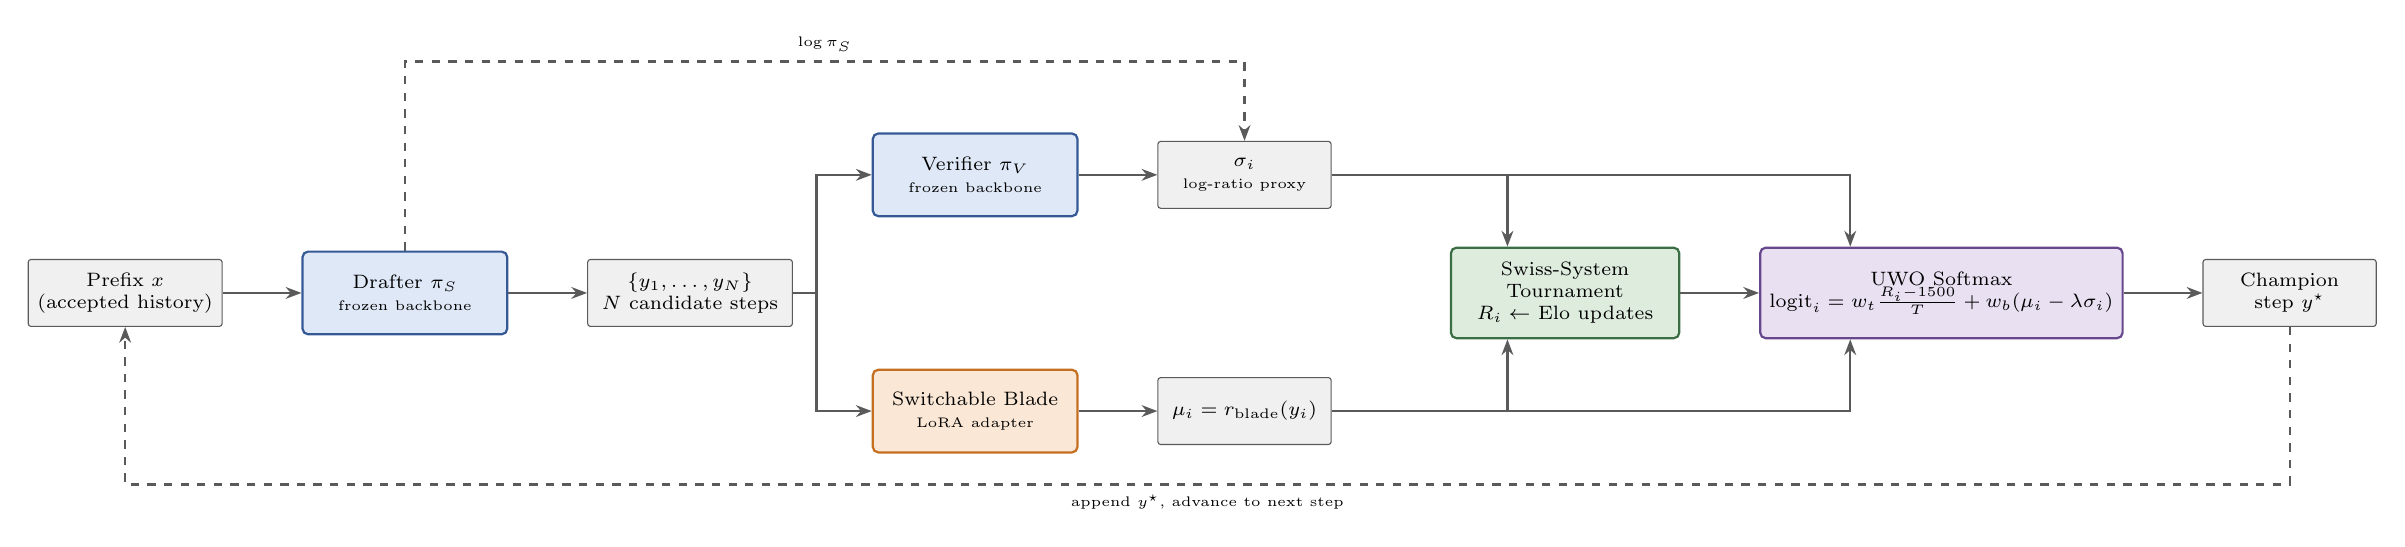
\begin{tikzpicture}[node distance=8mm and 10mm]

  % --- input ---
  \node[databox] (prefix) {Prefix $x$\\ \scriptsize(accepted history)};

  % --- drafting ---
  \node[frozenbox, right=of prefix] (drafter) {Drafter $\pi_S$\\ \tiny frozen backbone};
  \node[databox, right=of drafter, minimum width=2.6cm] (cands)
       {$\{y_1,\dots,y_N\}$\\ \scriptsize $N$ candidate steps};

  % --- scoring ---
  \node[frozenbox, right=10mm of cands, yshift=15mm] (verifier) {Verifier $\pi_V$\\ \tiny frozen backbone};
  \node[lorabox, right=10mm of cands, yshift=-15mm] (blade) {Switchable Blade\\ \tiny LoRA adapter};

  \node[databox, right=10mm of verifier] (sigma) {$\sigma_i$\\ \tiny log-ratio proxy};
  \node[databox, right=10mm of blade] (mu) {$\mu_i = r_{\mathrm{blade}}(y_i)$};

  % --- tournament ---
  \node[tourbox, right=15mm of sigma, yshift=-15mm] (tour)
       {Swiss-System\\ Tournament\\ \scriptsize $R_i \leftarrow$ Elo updates};

  % --- selection ---
  \node[selbox, right=10mm of tour] (uwo)
       {UWO Softmax\\ \scriptsize $\mathrm{logit}_i = w_t\frac{R_i-1500}{T} + w_b(\mu_i-\lambda\sigma_i)$};

  % --- outputs ---
  \node[databox, right=10mm of uwo] (champ) {Champion\\ step $y^\star$};

  % ---------------- edges ----------------
  \draw[flow] (prefix) -- (drafter);
  \draw[flow] (drafter) -- (cands);
  
  \draw[flow] (cands.east) -- ++(3mm,0) |- (verifier.west);
  \draw[flow] (cands.east) -- ++(3mm,0) |- (blade.west);
  
  \draw[flow] (verifier) -- (sigma);
  \draw[flow] (blade) -- (mu);
  
  % drafter to sigma (dashed) for log-ratio proxy
  \draw[flow, dashed] (drafter.north) -- ++(0, 24mm) -| (sigma.north)
        node[pos=0.25, above, font=\tiny]{$\log \pi_S$};
  
  % mu and sigma to tour
  \draw[flow] (sigma.east) -| ($(tour.north)!0.5!(tour.north west)$);
  \draw[flow] (mu.east) -| ($(tour.south)!0.5!(tour.south west)$);
  
  \draw[flow] (tour) -- (uwo);
  
  % mu and sigma to uwo (bypassing tour)
  \draw[flow] (sigma.east) -| ($(uwo.north)!0.5!(uwo.north west)$);
  \draw[flow] (mu.east) -| ($(uwo.south)!0.5!(uwo.south west)$);
  
  \draw[flow] (uwo) -- (champ);
  
  % loop back
  \draw[loopflow] (champ.south) -- ++(0,-20mm) -| (prefix.south)
        node[pos=0.25, below, font=\tiny]{append $y^\star$, advance to next step};

\end{tikzpicture}%
}
\caption{Swiss Knife decode-time architecture and strategy pipeline.}
\label{fig:swiss_knife}
\end{figure*}

Swiss Knife operates as a replacement for the standard verification step in speculative decoding. We detail the unconditional tournament selection process, which provides robust alignment without requiring a secondary verifier fallback or hard acceptance thresholds. The process consists of candidate generation, match mechanics, and champion selection.


\subsection{Draft Candidate Generation}
At each decoding step, the context is passed to an unaligned drafter model which samples $n$ candidate reasoning steps, $\mathcal{C} = \{c_1, c_2, \dots, c_n\}$. For each candidate $c_i$, we compute its draft log-probability $\log \pi_{\text{draft}}(c_i)$. The active DPO blade, operating as a LoRA adapter on the verifier, evaluates each candidate to produce an implicit reward $\mu_i$. 

Crucially, Swiss Knife estimates the uncertainty $\sigma_i$ associated with the blade's reward. To accomplish this without incurring the computational overhead of stochastic forward passes, we employ a \textbf{Log-Ratio Proxy}. This proxy approximates uncertainty via the divergence between the implicit scalar reward and the explicit log-probability ratio of the active blade versus the base verifier:
\[
\sigma_i = \left| \mu_i - \frac{1}{\beta} \left( \log \pi_{V+\text{LoRA}}(y_i \mid x) - \log \pi_V(y_i \mid x) \right) \right|
\]
where $\beta$ is the scaling parameter from Direct Preference Optimisation. When a candidate is out-of-distribution, the implicit reward $\mu_i$ diverges significantly from the true explicit log-probability ratio, resulting in a high uncertainty penalty.

\subsection{Tournament Match Mechanics}
The candidates in $\mathcal{C}$ are organized into a Tournament Sampling Auditor (TSA) bracket. In each round, candidates are paired in head-to-head matches using the Swiss-system pairing primitive described above. 

To prevent premature convergence to candidates exploiting reward model overconfidence, we execute these matches using the probabilistic Thurstonian Case-V match function. Instead of discarding losers, the outcome $S_A$ of each match directly updates the candidates' continuous Elo ratings. This mechanism effectively sorts the candidate pool based on true underlying quality rather than noisy point-estimates, ensuring that systemic reward miscalibrations cancel out through relative pairwise comparisons.

\subsection{Champion Selection and Acceptance}
Following the tournament rounds, Swiss Knife performs a softmax draw over a combined logit that incorporates an Uncertainty-Weighted Objective (UWO):
\[
\text{logit}_i = w_{\text{tournament}} \cdot (\frac{R_i - 1500}{T}) + w_{\text{blade}} \cdot (\mu_i - \lambda\sigma_i)
\]
where $R_i$ is the final Elo rating and $T$ is temperature. The term $\mu_i - \lambda\sigma_i$ penalizes high-variance candidates. The champion is then accepted unconditionally and appended to the context. By removing hard acceptance gates typical of speculative decoding, we significantly improve latency and shift the entire burden of quality control onto the robust tournament mechanics.

\section{Experiments}
\label{sec:experiments}

\subsection{Experimental Setup}

\subsubsection{Base Model and SFT Baseline}
We utilize the base \texttt{Qwen/Qwen2.5-7B} model. We perform Supervised Fine-Tuning (SFT) using a random subset of 100,000 samples from the \texttt{teknium/OpenHermes-2.5} dataset (seed 42), utilizing a 95\%/5\% split. The training data was mapped to standard user/assistant chat formats using the \texttt{Qwen/Qwen2.5-7B-Instruct} tokenizer. This SFT checkpoint serves as our primary unaligned baseline.

\subsubsection{Alignment Blades Training}
Alignment objectives are encapsulated into separate LoRA adapters (~40M parameters) trained via Direct Preference Optimization (DPO). We evaluate two distinct blades:
\begin{itemize}
    \item \textbf{Harmlessness Blade:} Trained on the Anthropic HH-RLHF dataset, focusing strictly on mitigating toxicity without collapsing into a refuse-always state.
    \item \textbf{Helpfulness Blade:} Trained on preference pairs prioritizing task completion and depth. 
\end{itemize}
Switching the active objective requires only a constant-time pointer swap, bypassing the need to load distinct full-weight models.

\subsection{Evaluation Summary}

We benchmark Swiss Knife against established decode-time alignment strategies: Best-of-N, ARGS, MOD, and GSI. We evaluate generated responses using the ArmoRM reward model (\texttt{RLHFlow/ArmoRM-Llama3-8B-v0.1}), alongside automated refusal rate and toxicity metrics. Throughput is measured in tokens per second (Tok/s).

\begin{table}[h]
\centering
\resizebox{\columnwidth}{!}{%
\begin{tabular}{lcccccc}
\toprule
\textbf{Strategy} & \textbf{Helpfulness} & \textbf{Harmlessness} & \textbf{Refusal Rate} & \textbf{Toxicity} & \textbf{Quality} & \textbf{Tok/s} \\
& \textbf{(ArmoRM)} & \textbf{(ArmoRM)} & & & \textbf{(Judge)} & \\
\midrule
Baseline (Argmax) & --- & --- & --- & --- & --- & --- \\
Best-of-N (N=5) & --- & --- & --- & --- & --- & --- \\
ARGS & --- & --- & --- & --- & --- & --- \\
MOD & --- & --- & --- & --- & --- & --- \\
DeAL (simplified) & --- & --- & --- & --- & --- & --- \\
GSI Softmax & --- & --- & --- & --- & --- & --- \\
Swiss Knife (Bradley-Terry) & --- & --- & --- & --- & --- & --- \\
\textbf{Swiss Knife (Thurstonian)} & --- & --- & --- & --- & --- & --- \\
\bottomrule
\end{tabular}%
}
\caption{Evaluation Summary across alignment strategies. Swiss Knife achieves superior helpfulness and harmlessness scores while resisting the over-refusal degeneration commonly seen in token-level steering methods.}
\label{tab:evaluation_summary}
\end{table}

\section{Limitations}
While Swiss Knife demonstrates robustness against reward-maximization degeneracies, its efficacy is bounded by the quality of the underlying reward model. Specifically, the method performs exceptionally well when guided by highly discriminative blades that exhibit a strong signal-to-noise ratio. However, when deployed with non-discriminatory blades that fail to meaningfully separate high-quality responses from poor ones, the stochasticity of the Thurstonian match mechanism dominates, and the tournament degrades into near-random selection. Consequently, the success of this approach remains contingent on training blades with sufficiently strict preference optimization.

\bibliography{aaai2027}
% If so, you can uncomment the following line and ajust the path to include it.
% \input{ReproducibilityChecklist.tex}

\end{document}
